% !TEX root = ../my-thesis.tex
%
\chapter{Search for dark matter in association with a dark Higgs boson decaying to \(b\)-quarks}
\label{ch:monoSbb}

\section{Introduction}
\label{sec:monoSbb:introduction}
This chapter describes the search for dark matter in association with a dark Higgs boson \(s\).
The signature of missing transverse momentum and a hypothetical dark Higgs boson is predicted by the 2MDM simplified model (c.f.~\Cref{sec:dm:models:2mdm}). The presence of such a dark Higgs boson is motivated both by the need to generate the masses of dark matter particles and the \PZprime boson mediator and by constraints on models of dark matter production due to the observed dark matter relic density~\cite{Duerr2017}.

The dark Higgs boson can mix with the SM Higgs boson and thereby shares its decay modes. Consequently, the dark Higgs boson can be sought by searches in various final states, which probe a broad dark Higgs boson mass range.
The search presented in this chapter focuses on the dark Higgs boson decay to \bquarks and is sensitive to dark Higgs bosons in the mass range below \SI{160}{\giga\electronvolt}, while \Cref{ch:monoSVV} focuses on the decay to pairs of weak vector bosons and extends the coverage towards heavier dark Higgs boson signals.

The production of dark matter particles \(\chi\) in association with a dark Higgs boson decaying to \bquarks shares the signature of \met and two \btagged jets with the \(\met + \Hbb\) search, except for the mass of the Higgs boson candidate. The primary discriminating variable of the \(\met + \Hbb\) search is the invariant mass of the Higgs candidate, which extends from \SIrange{50}{280}{\giga\electronvolt}. Therefore, the search presented in \Cref{ch:monoH} can be reinterpreted in terms of the 2MDM simplified model for a dark Higgs boson signal with mass \ms.

The reinterpretation is performed using the RECAST framework (c.f. \Cref{sec:methods:recast}).
It is based on the 2015--2017 \HepProcess{\Pp\Pp} dataset corresponding to an integrated luminosity of \SI{79.8}{\per\femto\barn}.
Constraints on the 2MDM model are obtained by combining the preserved background model and observed data of the \(\met + \Hbb\) search with distributions of the discriminating variables for the simulated 2MDM signal model points.
While previous efforts already demonstrated capturing the analysis software in containers to be feasible~\cite{SUSY-2014-08,SUSY-2015-12,EXOT-2017-32,ATLAS-CONF-2018-003}, this reinterpretation also captures the analysis workflow and thereby is fully automated. The results of this reinterpretation have been presented in Ref.~\cite{ATL-PHYS-PUB-2019-032}.

\Cref{sec:monoSbb:physics} introduces the signal process in the search for dark matter and dark Higgs bosons decaying to \bquarks. As this search is a reinterpretation of the \(\met + \Hbb\) search, the background processes are the same as those described in \Cref{sec:monoH:physics:backgrounds}.
The systematic uncertainties on the signal are discussed in \Cref{sec:monoSbb:systematics}. The technical implementation in the RECAST framework is described in \Cref{sec:monoSbb:implementation}, while the results are presented in \Cref{sec:monoSbb:results}. A conclusion is given in \Cref{sec:monoSbb:conclusion}.


\section{Signal processes}
\label{sec:monoSbb:physics}
The analysis investigates dark matter production in the framework of the 2MDM simplified model, which is described in \Cref{sec:monoSbb:physics:2mdm}. The simulated signal samples are summarised in \Cref{sec:monoSbb:physics:mcsamples}.

\subsection{2MDM simplified model}
\label{sec:monoSbb:physics:2mdm}
The 2MDM simplified model is considered for the reinterpretation of the \(\met + \Hbb\) search. It is a simplified model in which a \PZprime spin-1 mediator and a dark Higgs boson \(s\) arise from a spontaneously broken \(\text{U}(1)_{\PZprime}\) gauge symmetry and an additional complex Higgs field (c.f. \Cref{sec:dm:models:2mdm}).

The processes yielding the signature of \(\met + \sbb\) are illustrated by the two example Feynman graphs in \Cref{fig:monoSbb:physics:2mdm:graph}.

\begin{figure}[hbtp]
  \centering
  \begin{subfigure}{.45\textwidth}
  	\centering
	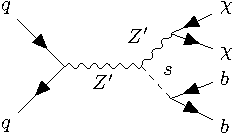
\includegraphics[width=0.85\textwidth]{figures/monoS/physics/monos1.pdf}
    \caption{}
  \end{subfigure}
  \begin{subfigure}{.45\textwidth}
    \centering
    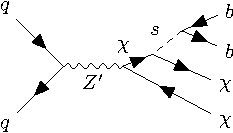
\includegraphics[width=0.85\textwidth]{figures/monoS/physics/monos2.pdf}
    \caption{}
  \end{subfigure}
  \caption{Production of dark matter particles \(\chi\) and a dark Higgs boson \(s\) through \(s\)-channel exchange of a new \PZprime mediator. The dark Higgs boson is decaying to \bquarks.}
  \label{fig:monoSbb:physics:2mdm:graph}
\end{figure}

A \PZprime vector boson is produced in \HepProcess{\Pp\Pp} collisions, which couples both to dark matter particles and the dark Higgs boson. The dark Higgs boson can be radiated off either from the \PZprime boson or from a dark matter particle in the final state. Through mixing with the SM Higgs boson, the dark Higgs boson decays to visible particles, such as \bquarks or weak vector bosons.

The relevant model parameters and their chosen values are listed in \Cref{tab:monoSbb:physics:2mdm:parameters}. These parameters include the masses of the involved particles \mZp, \ms, \mchi, the gauge couplings of the \PZprime boson to quarks \gq and the dark sector \gchi, and the mixing angle between the SM Higgs boson and the dark Higgs boson. The dark matter particle mass \mchi is set to \SI{200}{\giga\electronvolt}.
The chosen values of the couplings \(\gq = 0.25\) and \(\gchi = 1\) are adopted to allow for comparisons with other simplified models, despite stringent constraints on \gq from dijet searches~\cite{EXOT-2017-32}. The mixing angle between the dark Higgs boson and the SM Higgs boson is set to \(\theta = 0.01\), following the choice adopted in Ref.~\cite{Duerr2017}.

The interpretation of the results of the search is performed via a scan over the two-dimensional \mZp-\ms plane for fixed choices of the coupling parameters and the dark matter mass \(\mchi = \SI{200}{\giga\electronvolt}\). The scan extends over the range \SIrange{500}{3500}{\giga\electronvolt} in \mZp and \SIrange{50}{150}{\giga\electronvolt} in \ms.

\begin{table}[htbp]
\caption{Parameters of the 2MDM simplified model in the searches for dark matter in association with a dark Higgs boson.}
\label{tab:monoSbb:physics:2mdm:parameters}
\centering
\begin{tabular}{l l r}
\toprule
Parameter & Description & Chosen value \\
\midrule
\mZp & \PZprime boson mass & free \\
\ms & dark Higgs boson mass & free \\
\mchi & dark matter particle mass & \SI{200}{\giga\electronvolt}\\
\gq & \PZprime gauge coupling to quarks & \num{0.25} \\
\gchi & \PZprime gauge coupling to the dark sector & \num{1} \\
\(\theta\) & mixing angle between the SM Higgs boson & \num{0.01} \\
           & and the dark Higgs boson & \\
\bottomrule
\end{tabular}
\end{table}


\subsection{Simulated Monte Carlo samples for signal processes}
\label{sec:monoSbb:physics:mcsamples}
Signals of the process \HepProcess{\Pp\Pp \to \PZprime \to \chi \overline{\chi} + \Pqb \Paqb } are simulated by scanning the mass of the \PZprime boson in the range \SIrange{500}{3500}{\giga\electronvolt} in steps of \SI{500}{\giga\electronvolt} and the mass of the dark Higgs boson \ms in the range \SIrange{50}{150}{\giga\electronvolt} in \SI{20}{\giga\electronvolt} steps.

The simulated events are generated at leading-order (\LO) accuracy with the \MGMCatNLOV{2.6.2} event generator~\cite{Alwall:2014hca} interfaced to the \PYTHIAV{8.230}~\cite{Sjostrand:2014zea} parton shower and hadronisation model, using the \textsc{NNPDF23} PDF set~\cite{Ball:2012cx} and the \AFourteen set of tuned parameters~\cite{ATL-PHYS-PUB-2014-021}.
To remove the overlap between the hard scattering and the parton shower model, the CKKW-L merging procedure~\cite{Lnnblad2002,Lnnblad2012} is applied with the matching scale set to \SI{40}{\giga\electronvolt}.



\section{Systematic uncertainties on the signal process}
\label{sec:monoSbb:systematics}
Only the systematic uncertainties associated with the signal process need to be estimated, as the preserved background model of the \(\met + \Hbb\) search already contains all systematic uncertainties on the background.

The experimental systematic uncertainties on the signal process are estimated similarly to those on the background process, using the calibration tools which are part of the preserved analysis software.

The theoretical systematic uncertainties on the signal process are estimated by varying the model parameters and
comparing the event yield after applying the analysis selection at particle level neglecting detector effects. Renormalisation and factorisation scale uncertainties and variations of parton distribution functions (PDFs) are considered in the four \met bins of the search. The scale uncertainties in individual \met bins range from \SIrange{6.2}{22.2}{\percent}, while the uncertainty on PDFs ranges from \SIrange{3.8}{16.4}{\percent}.
The signal acceptance uncertainties are correlated over the \met bins by considering a single nuisance parameter for each type of systematic uncertainty.


\section{Technical implementation}
\label{sec:monoSbb:implementation}
The reinterpretation requires the simulated events for the 2MDM simplified model signals to be processed by the analysis workflow, which consists of two steps. The first step involves processing the simulated events for the signal process to obtain fit inputs for the statistical inference. The second step combines these inputs with the preserved background estimate and the observed data of the \(\met + \Hbb\) search to compute upper limits on the signal strength of the 2MDM simplified model signals.
\Cref{fig:monoSbb:implementation:illustration} illustrates the workflow, which consists of the following steps:

\begin{figure}[htbp]
  \centering
  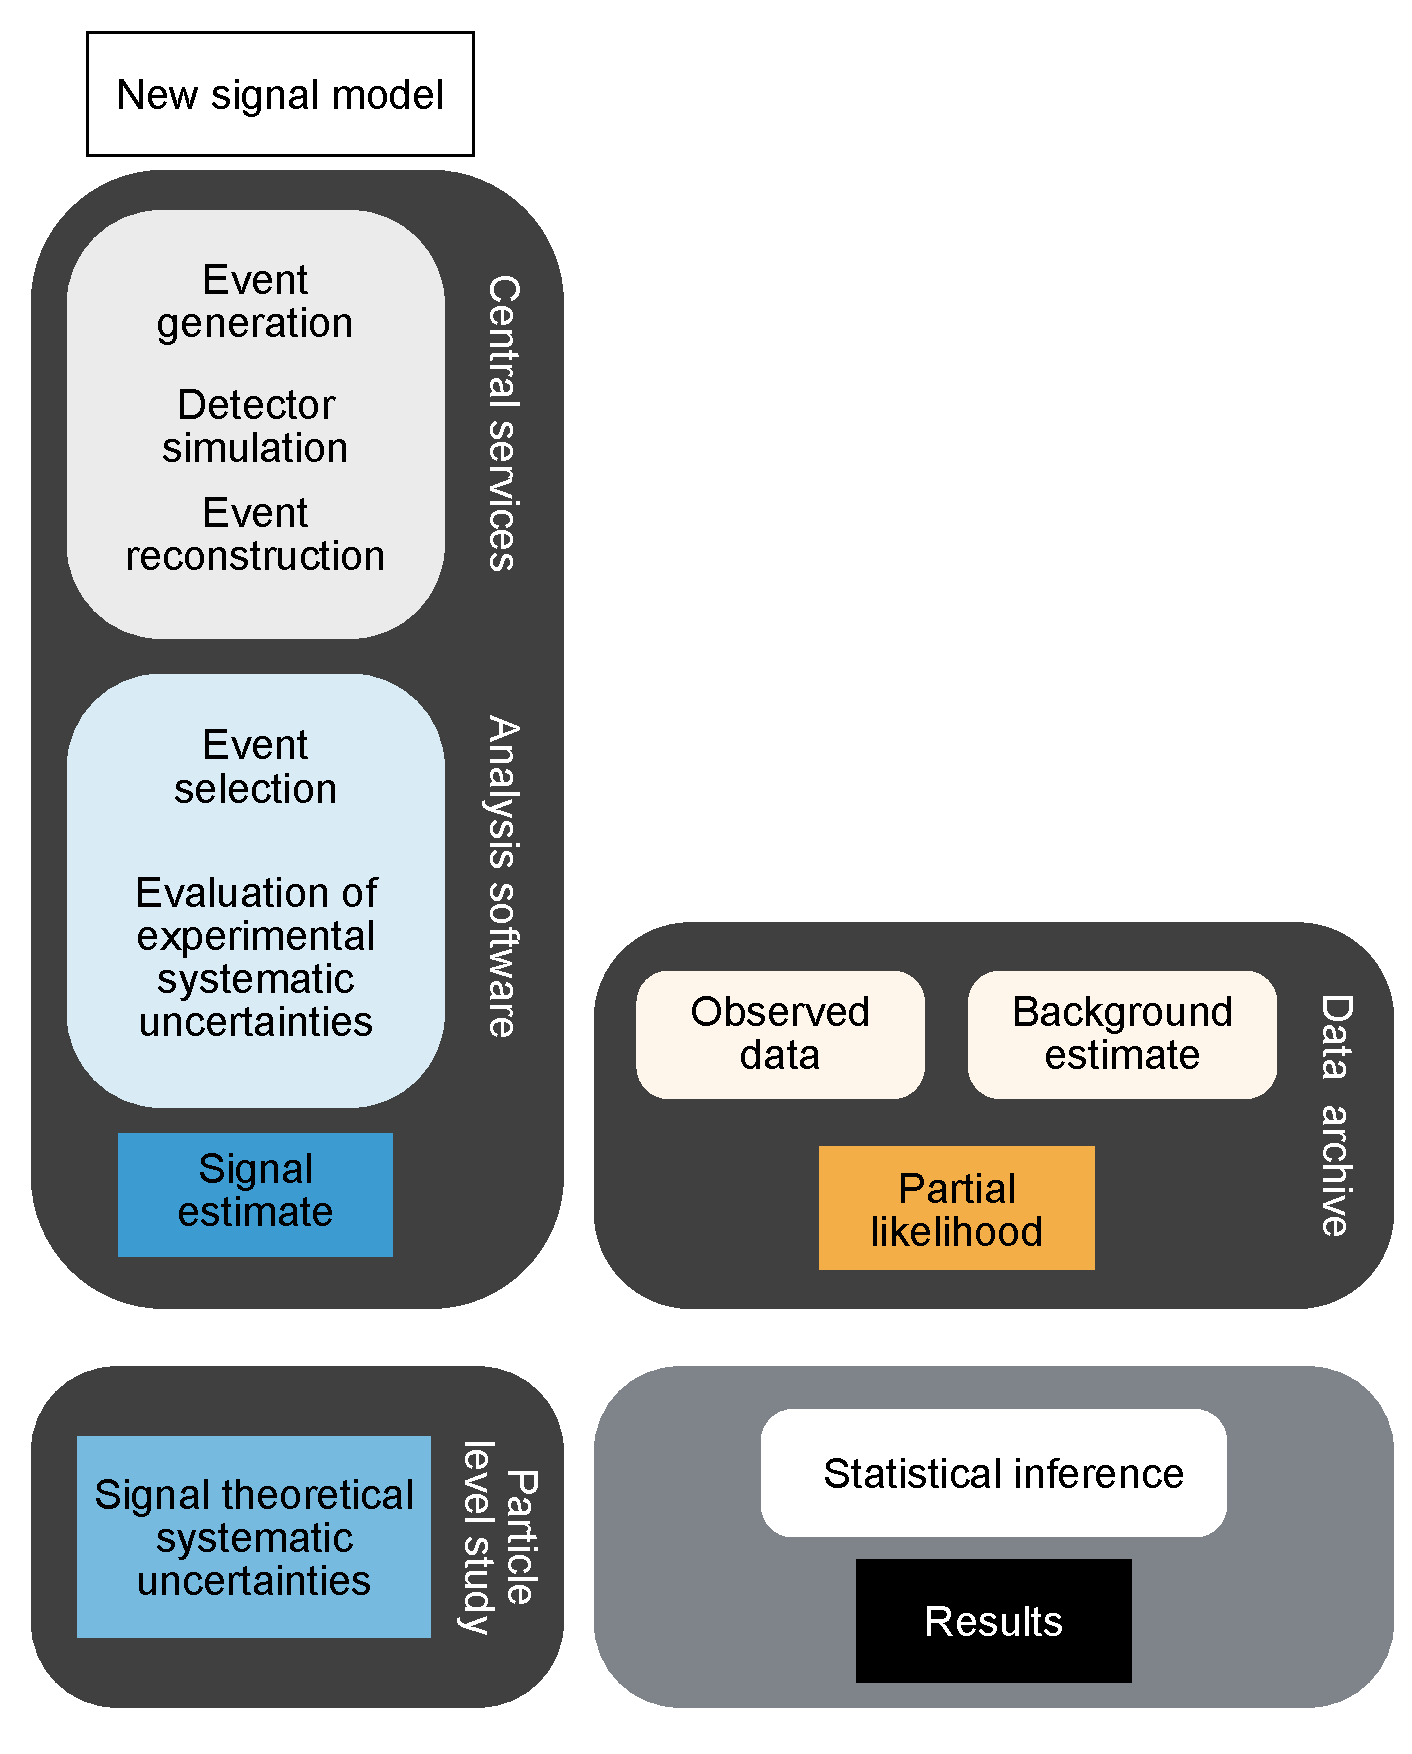
\includegraphics[width=0.95\textwidth]{figures/monoS/recast_workflow.pdf}
  \caption{Workflow for the RECAST reinterpretation of the \(\met + \Hbb\) search. The signal preparation step is performed using centrally provided services for MC event generation, detector simulation, and event reconstruction of the new signal sample. The signal analysis is based on the RECAST framework services by capturing the analysis software and the associated workflow for performing the event selection and the evaluation of experimental systematic uncertainties on the signal estimate. The statistical inference combines the partial likelihood, which is constructed using the preserved data and background estimate, the signal estimate, and the theoretical systematic uncertainties on the signal. The latter are estimated using a simplified implementation of the analysis on particle level neglecting detector effects.}
  \label{fig:monoSbb:implementation:illustration}
\end{figure}

\begin{itemize}
	\item \textbf{Signal preparation}. The signal events are sampled using the standard tools as described in \Cref{sec:common:data:mc}, which are centrally maintained and thus do not require the expert knowledge encoded in RECAST.
	\item \textbf{Signal analysis}. The event processing stage involves the calibration of physics objects, object and event selection, as well as the variation of the latent parameters in the simulation to account for systematic uncertainties. In addition, the pile-up profile of the simulated events is corrected to match the data, and the simulated events are weighted according to the integrated luminosity.
	This step is performed using a \textsc{Docker} image of the event processing software, which is maintained on the CERN GitLab~\cite{Hethey2013} platform. The output of the signal analysis step is the expected number of events in each SR \met bin, including the systematic uncertainty in the expected event yield.
	\item \textbf{Inference}. The statistical inference involves the construction of a binned likelihood following \Cref{eq:methods:statistics:likelihood}. The preserved background and data inputs are combined with the newly derived signal estimates. As the predicted signal yields are estimated using simulation, they are subject to systematic uncertainties on the acceptance. The likelihood function accounts for this through the addition of nuisance parameters and corresponding constraint terms. Upper limits on the signal cross-section normalised to the theoretical expectation are derived from the constructed likelihood.
\end{itemize}


\section{Results}
\label{sec:monoSbb:results}
The results of the \(\met + \Hbb\) search established that the observed data is compatible with the SM background, and no significant excess has been observed. Therefore, exclusion limits on the 2MDM signal model are placed in the statistical inference step of the reinterpretation, which is based on the same combined profile likelihood fit as in the \(\met + \Hbb\) search, only with the signal and its associated uncertainties replaced.

\Cref{fig:monoSbb:results:met} shows the \met distribution for the observed data corresponding to an integrated luminosity of \SI{79.8}{\per\femto\barn} and the expected SM background before and after the background-only fit.

\begin{figure}[htbp]
\centering
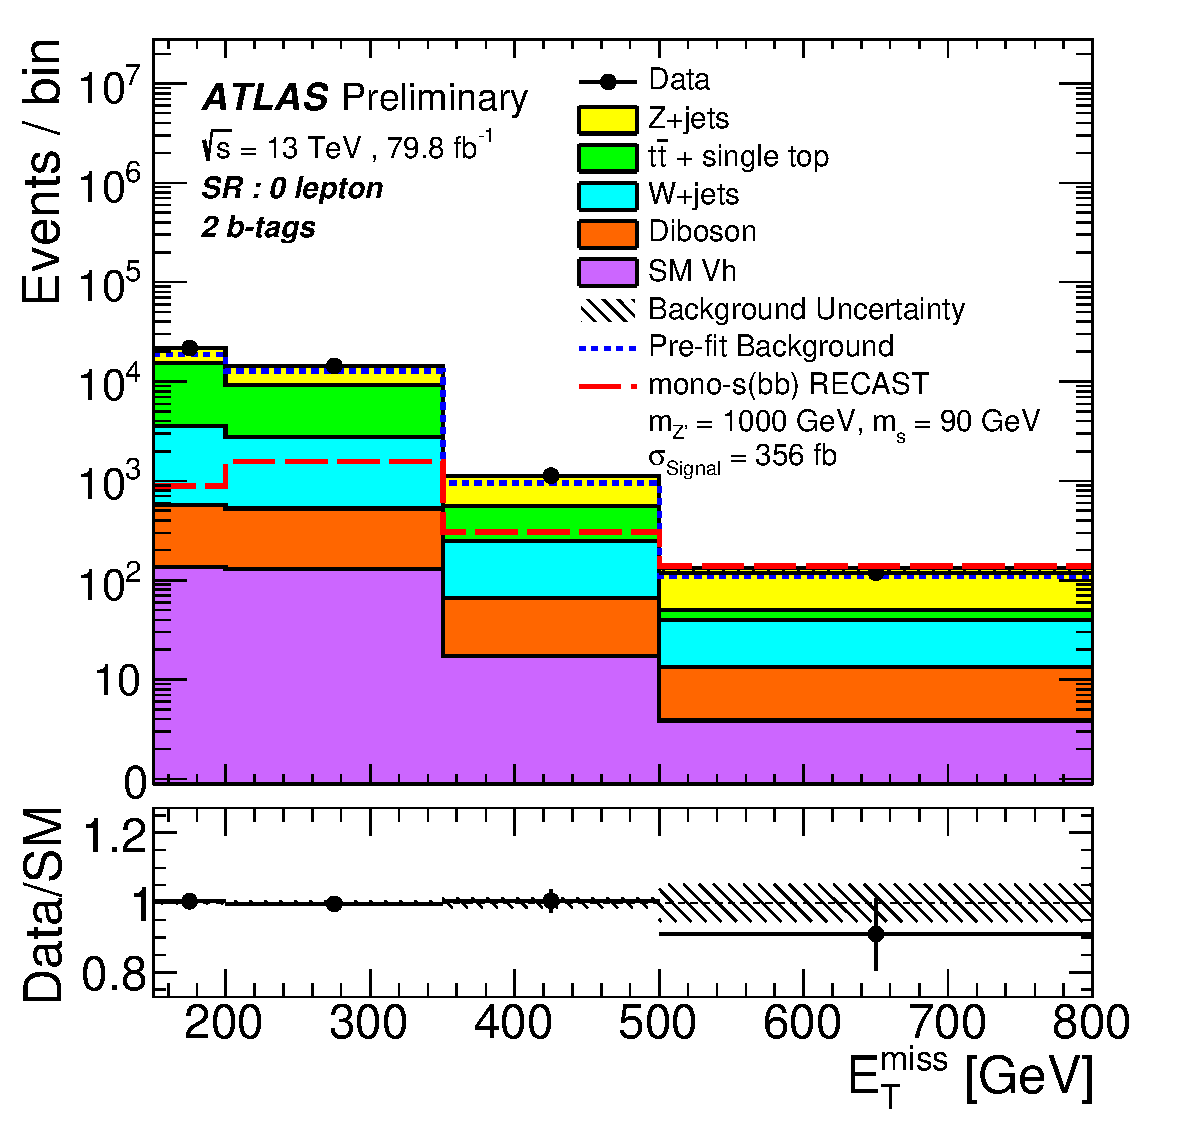
\includegraphics[width=0.95\textwidth]{figures/monoS/recast/fig_03.pdf}
\caption{\met distribution for the SR. The upper panel shows the comparison of data to the SM background expectation before~(dashed lines) and after the background-only fit~(solid histograms). The expected distribution for a representative 2MDM signal with \(\mZp = \SI{1}{\tera\electronvolt}\) and \(\ms = \SI{90}{\giga\electronvolt}\) is overlaid~(long-dashed line). The signal is scaled to an arbitrary cross-section of \SI{356}{\femto\barn} for visualisation. The lower panel shows the ratio of data to SM background expectations after the background-only fit, with the hatched band showing the systematic uncertainty.}
\label{fig:monoSbb:results:met}
\end{figure}

The invariant mass distributions in the SR are shown in \Cref{fig:monoSbb:results:mass}.
The distributions are exactly the same as those shown in \Cref{fig:monoH:results:observed:met}, except for the new signal process (red dashed line), which corresponds to the production of a dark Higgs boson with mass \(\ms = \SI{90}{\giga\electronvolt}\) via a \PZprime boson mediator with \(\mZp = \SI{1}{\tera\electronvolt}\).
The signal process is characterised by a mass peak at \((m_{jj}\) and \(m_{J} = \SI{90}{\giga\electronvolt}\), which becomes more evident with increasing \met due to the decreasing contribution of background processes.

\begin{figure}[htbp]
\centering
  \begin{subfigure}{0.45\textwidth}
    \centering
    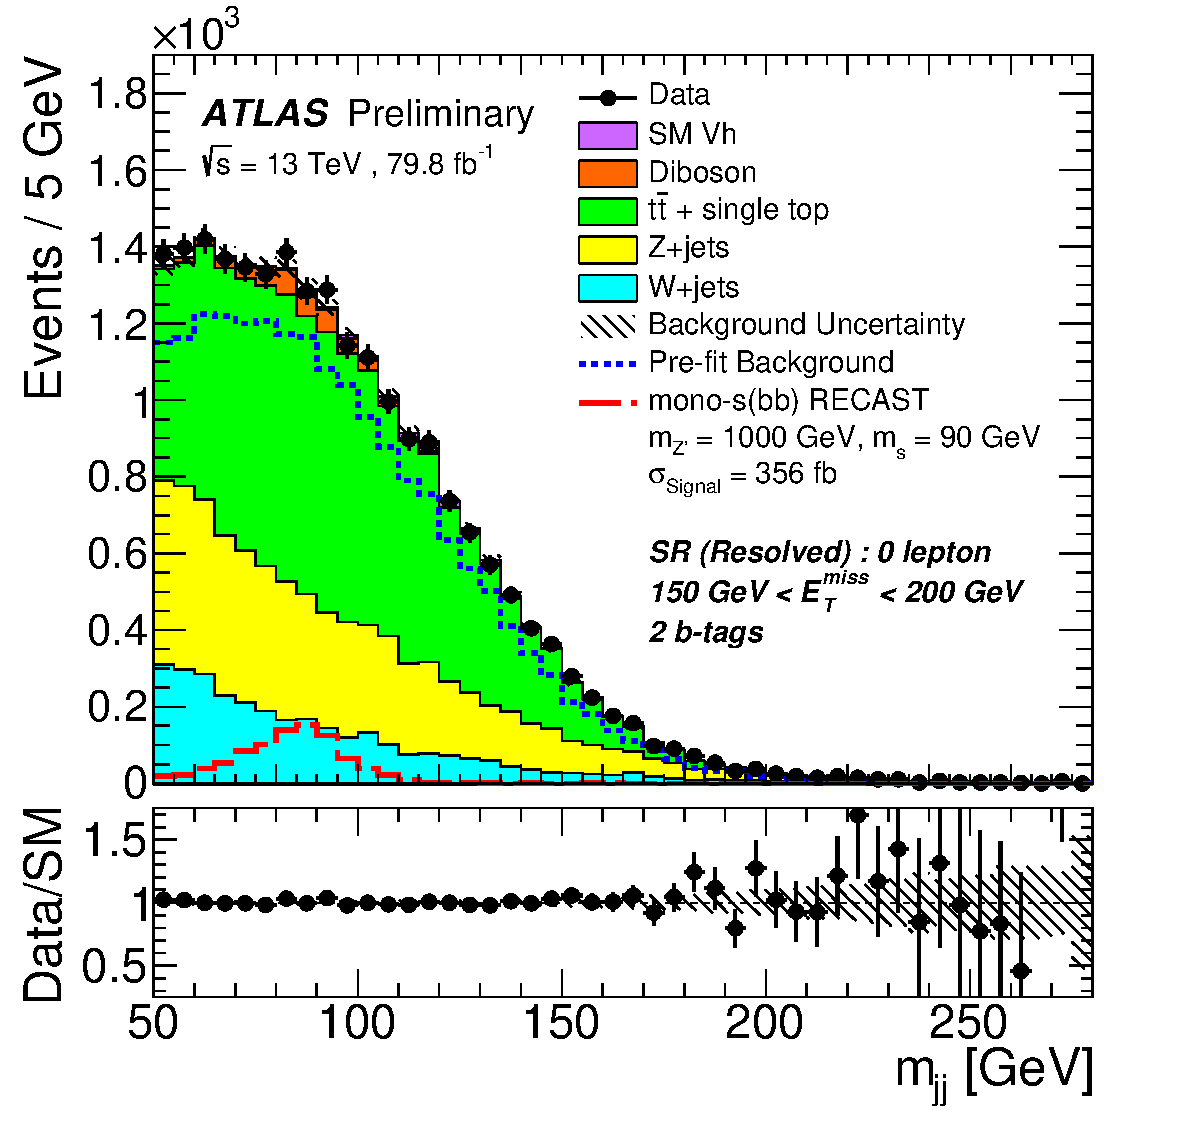
\includegraphics[width=0.95\textwidth]{figures/monoS/recast/fig_04a.pdf}
    \caption{SR resolved category \\\(\SI{150}{\giga\electronvolt} < \met < \SI{200}{\giga\electronvolt}\)}
  \end{subfigure}
  \begin{subfigure}{0.45\textwidth}
    \centering
    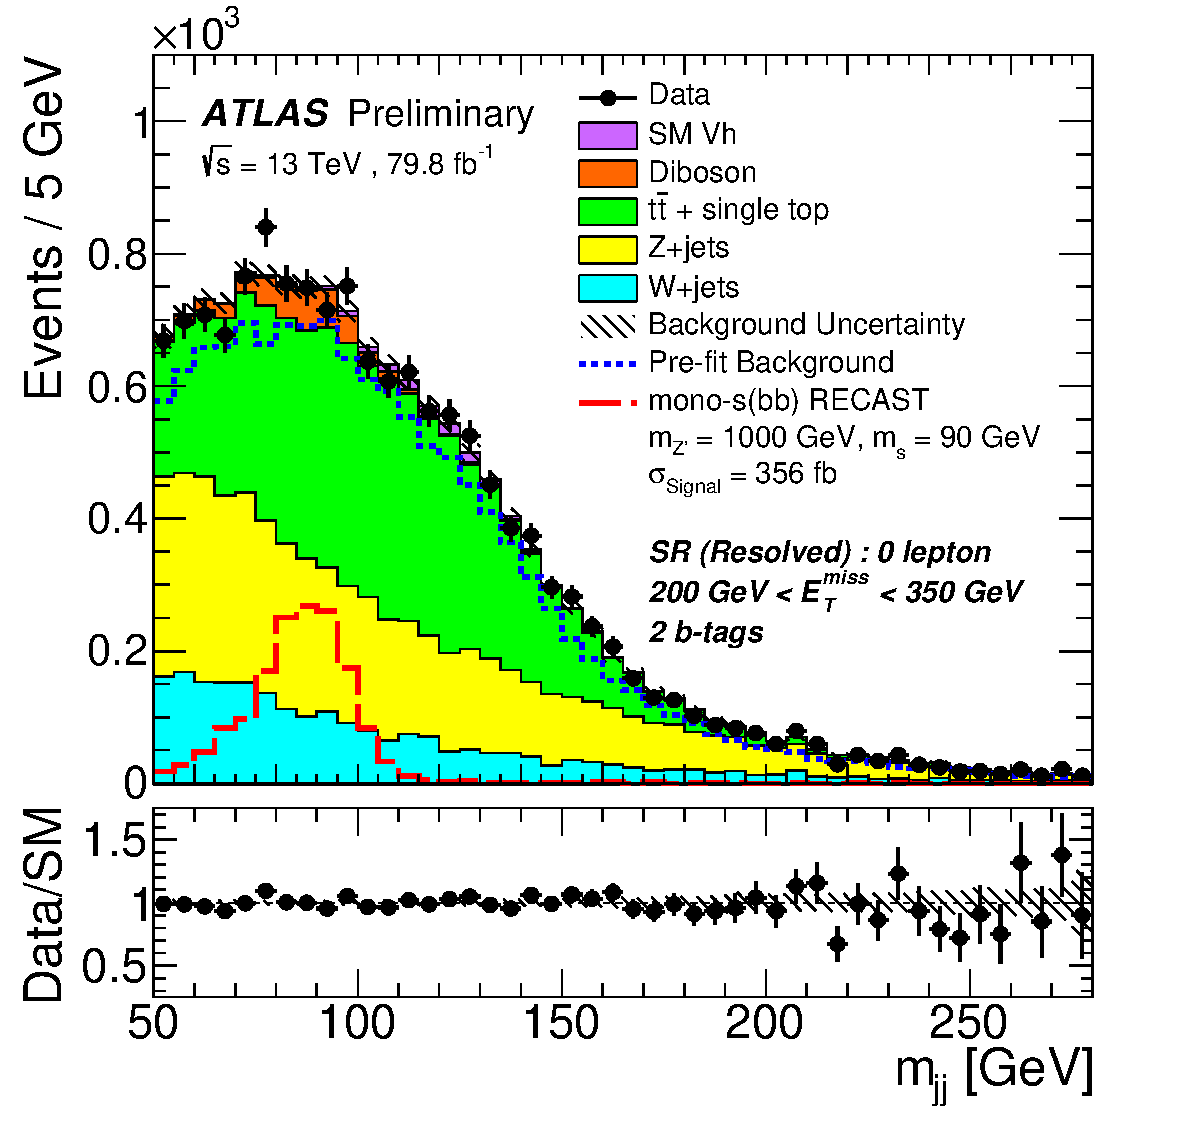
\includegraphics[width=0.95\textwidth]{figures/monoS/recast/fig_04b.pdf}
    \caption{SR resolved category \\\(\SI{200}{\giga\electronvolt} < \met < \SI{350}{\giga\electronvolt}\)}
  \end{subfigure}
  \\
  \begin{subfigure}{0.45\textwidth}
    \centering
    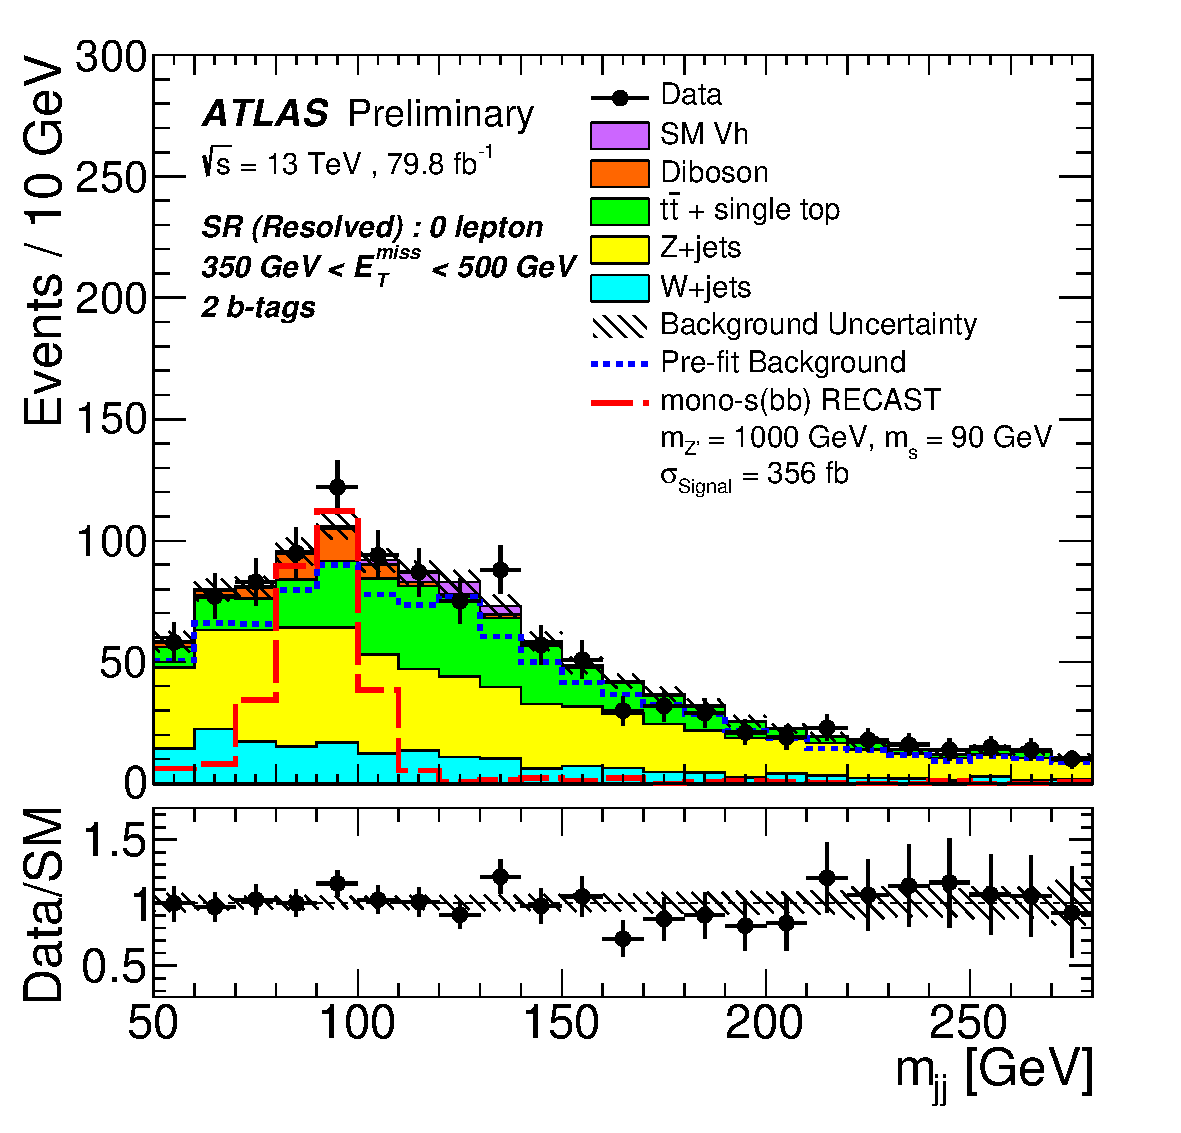
\includegraphics[width=0.95\textwidth]{figures/monoS/recast/fig_04c.pdf}
    \caption{SR resolved category \\\(\SI{350}{\giga\electronvolt} < \met < \SI{500}{\giga\electronvolt}\)}
  \end{subfigure}
  \begin{subfigure}{0.45\textwidth}
    \centering
    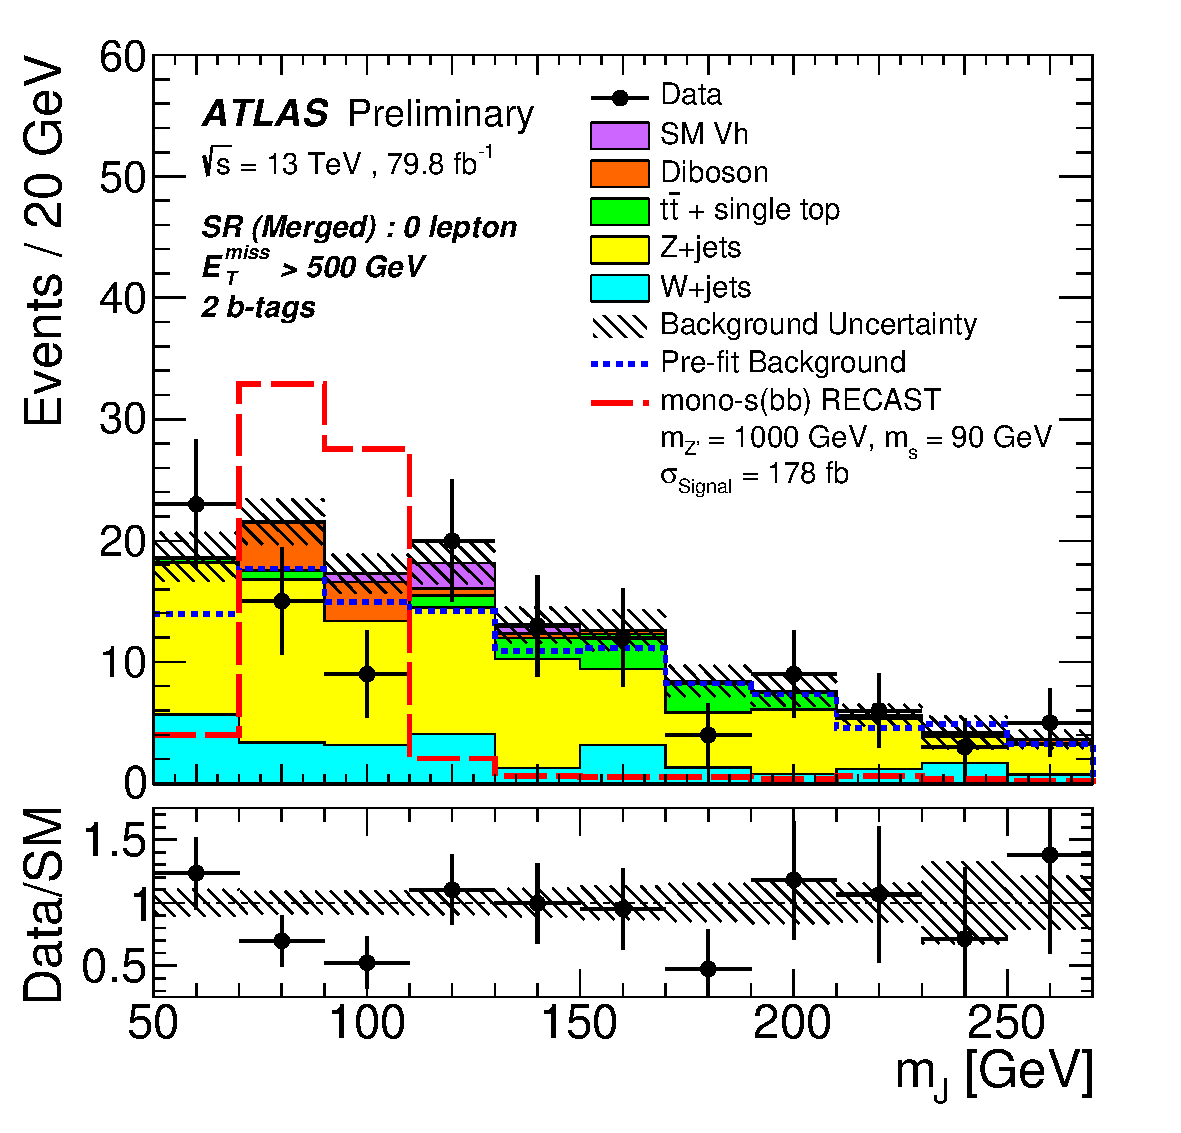
\includegraphics[width=0.95\textwidth]{figures/monoS/recast/fig_04d.pdf}
    \caption{SR merged category}
    \label{fig:monoSbb:results:mass:merged}
  \end{subfigure}
  \caption{Distributions of the Higgs boson candidate invariant mass \(m_{jj}\) (resolved), \(m_{J}\) (merged) in the SR for the four \met bins. The upper panels show a comparison of data to the SM expectation before~(dashed lines) and after the background-only fit~(solid histograms). The expected distribution for a representative 2MDM signal with \(\mZp = \SI{1}{\tera\electronvolt}\) and \(\ms = \SI{90}{\giga\electronvolt}\) is overlaid~(long-dashed line). The signal is scaled to an arbitrary cross-section of \SI{356}{\femto\barn} in the resolved category and \SI{178}{\femto\barn} in the merged category for visualisation. The lower panels show the ratio of data to SM background expectations after the background-only fit, with the hatched band indicating the systematic uncertainty.}
  \label{fig:monoSbb:results:mass}
\end{figure}

The expected and observed upper \SI{95}{\percent} \(\text{CL}_{s}\) limits on the signal strength \(\mu\) as a function of \mZp and \ms are shown in \Cref{fig:monoSbb:results:limits} for the fixed choice of parameters \(\mchi = \SI{200}{\giga\electronvolt}\), \(\gq = 0.25\), and \(\gchi = 1\). If the upper limit is below one, the specific model configuration is excluded at \SI{95}{\percent} \(\text{CL}_{s}\).

\begin{figure}[htbp]
\centering
  \begin{subfigure}{1.\textwidth}
    \centering
    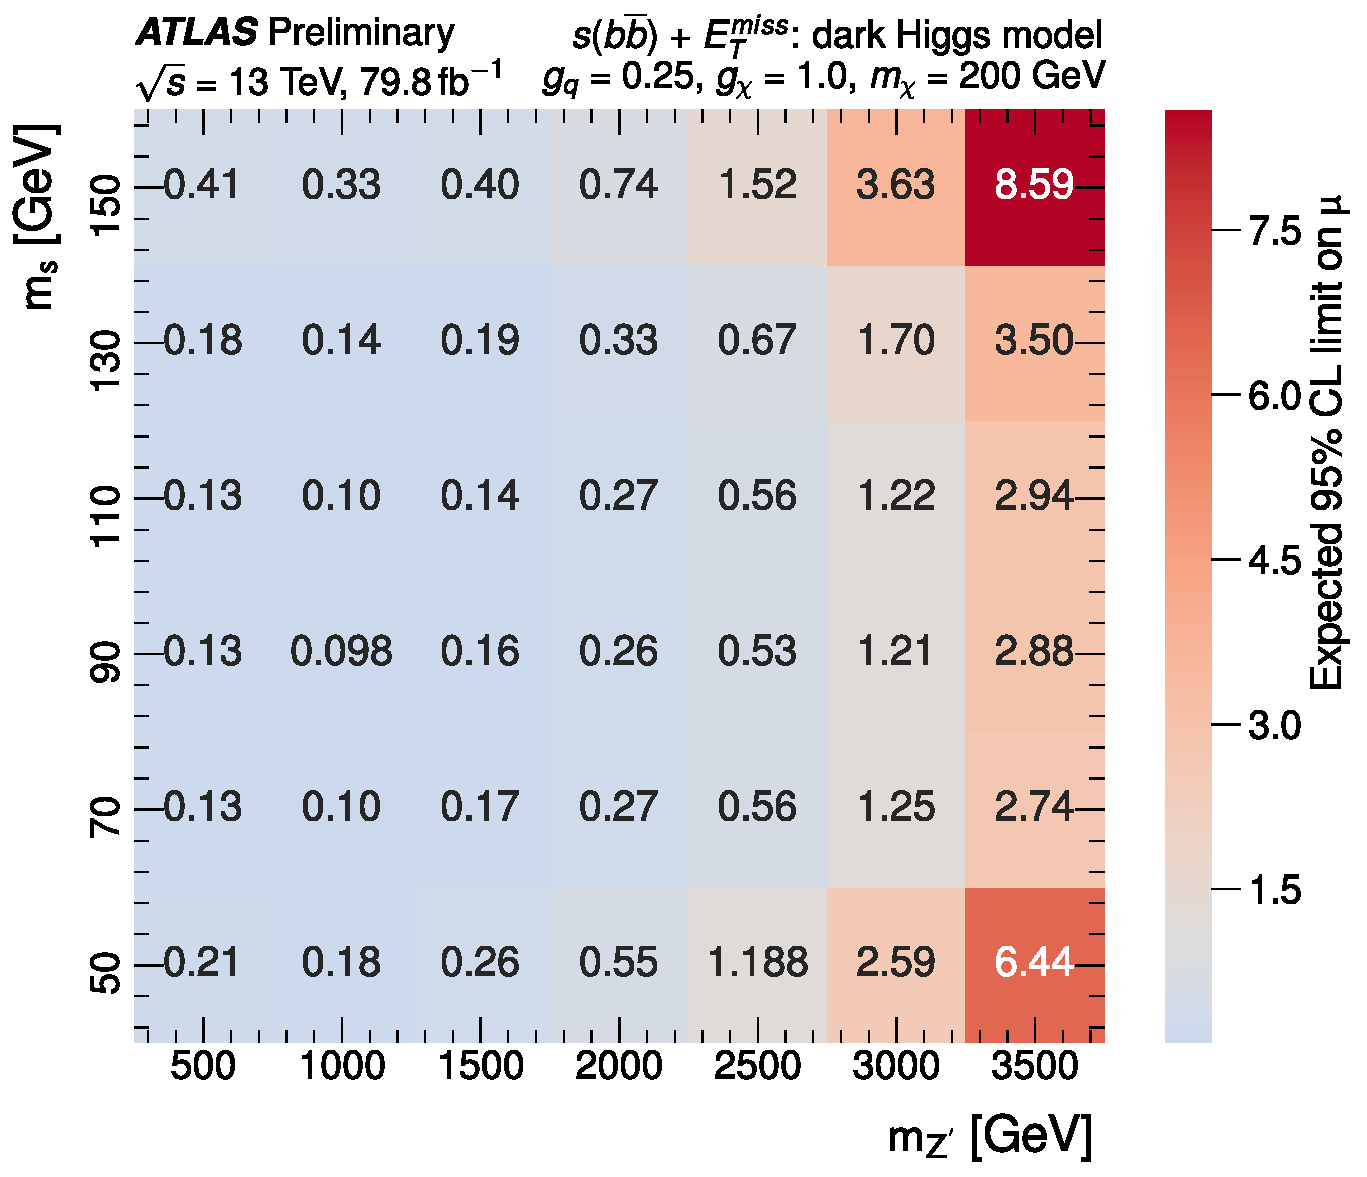
\includegraphics[width=0.75\textwidth]{figures/monoS/recast/fig_06a.pdf}
    \caption{Expected upper limits on the signal strength \(\mu\)}
  \end{subfigure}
  \\
  \begin{subfigure}{1.\textwidth}
    \centering
    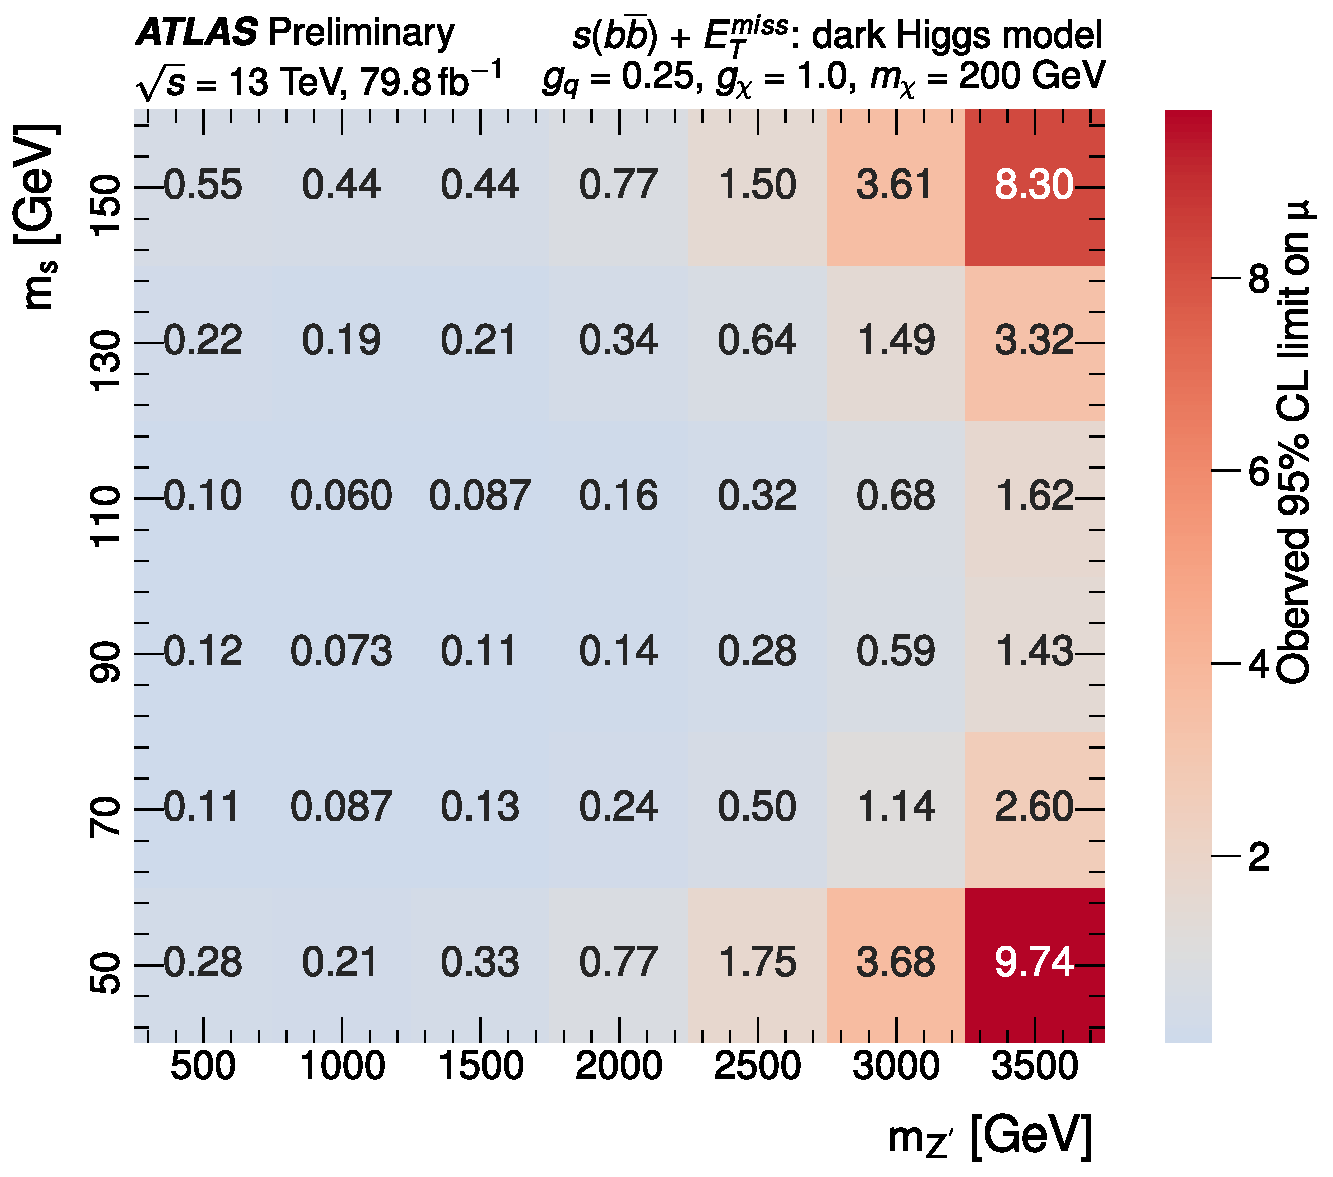
\includegraphics[width=0.75\textwidth]{figures/monoS/recast/fig_06b.pdf}
    \caption{Observed upper limits on the signal strength \(\mu\)}
  \end{subfigure}
  \caption{Upper \SI{95}{\percent} \(\text{CL}_{s}\) exclusion limits on the signal strength \(\mu\) for the 2MDM simplified model with parameters \(\mchi = \SI{200}{\giga\electronvolt}\), \(\gq = 0.25\), and \(\gchi = 1\) for different values of \mZp and \ms. The expected exclusion limits are shown at the top, while the observed exclusion limits are shown at the bottom.}
  \label{fig:monoSbb:results:limits}
\end{figure}

The exclusion limits can also be presented as a corresponding exclusion contour in the \mZp-\ms plane, as shown in \Cref{fig:monoSbb:results:contour}. The region to the left of the observed \SI{95}{\percent} \(\text{CL}_{s}\) exclusion contour, which is indicated by the black line, is excluded. The expected exclusion contour is indicated by the dashed line, while the green and yellow bands represent the \(\pm 1 \sigma\) and \(\pm 2 \sigma\) uncertainty, respectively.

\begin{figure}[htbp]
    \centering
    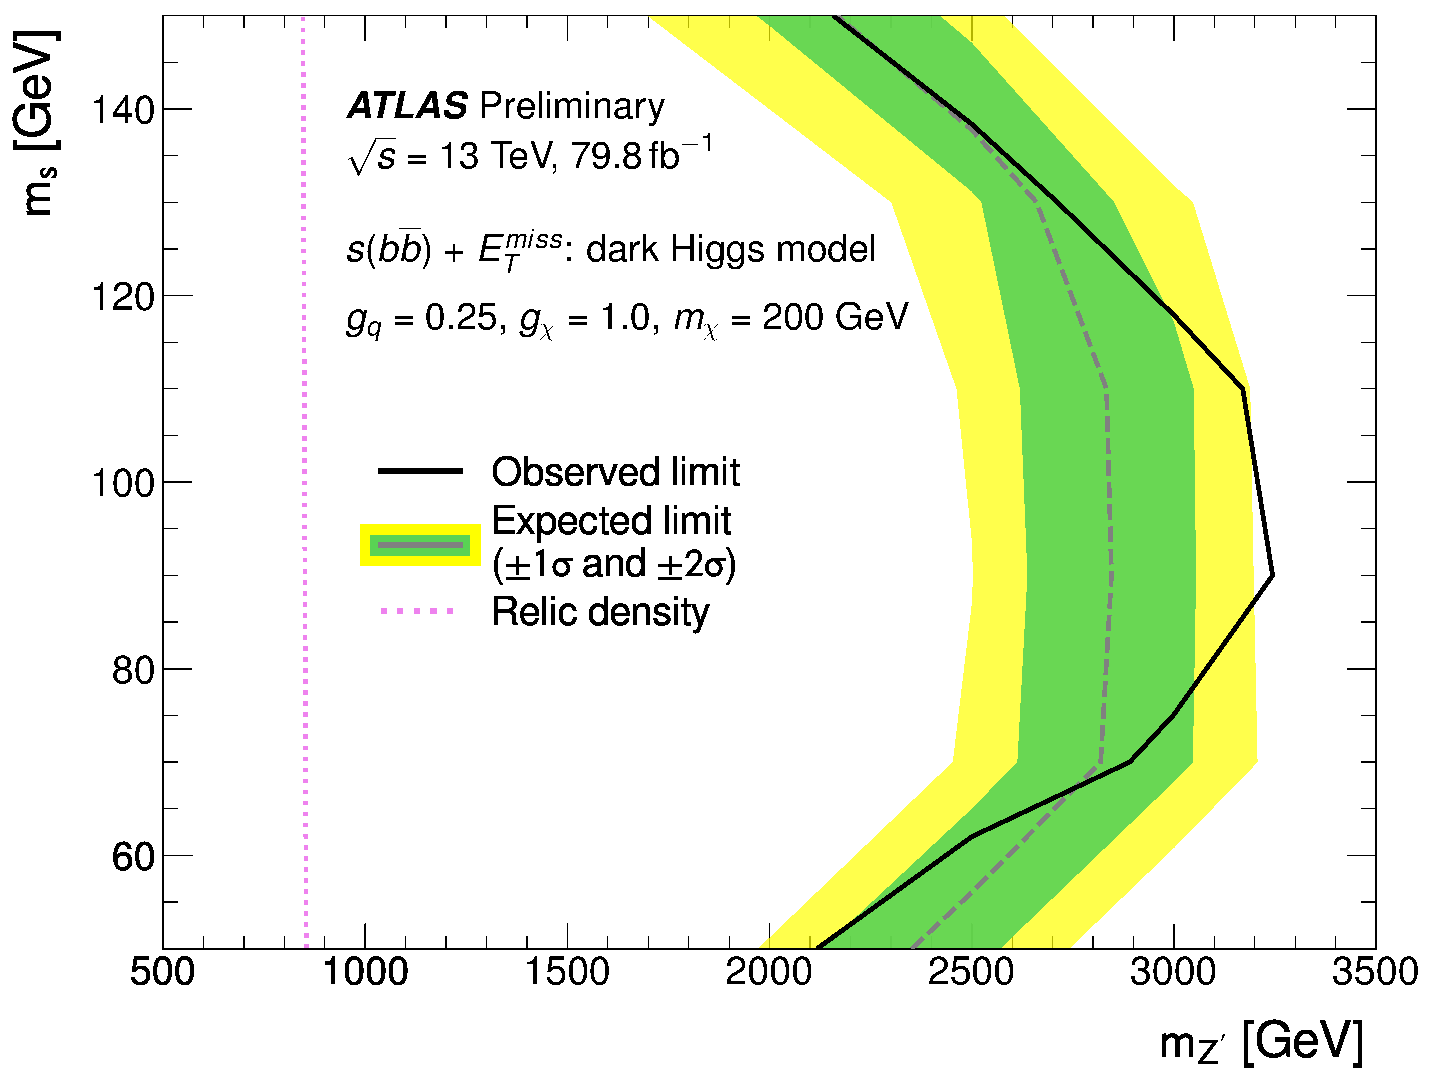
\includegraphics[width=.95\textwidth]{figures/monoS/recast/fig_07.pdf}
    \caption{Exclusion contours at \SI{95}{\percent} \(\text{CL}_{s}\) for the 2MDM simplified model in the \mZp-\ms plane for the fixed set of parameters \(\mchi = \SI{200}{\giga\electronvolt}\), \(\gq = 0.25\), and \(\gchi = 1\). The observed limits~(solid line) are consistent with the expectation under the SM-only hypothesis~(densely dashed line) mostly within \(\pm 2 \sigma\) uncertainties~(filled bands).}
    \label{fig:monoSbb:results:contour}
\end{figure}

The expected exclusion of the 2MDM parameter space for the fixed choice of parameters \(\mchi = \SI{200}{\giga\electronvolt}\), \(\gq = 0.25\), and \(\gchi = 1\) extends in \mZp up to \SI{2.3}{\tera\electronvolt} for \(\ms = \SI{50}{\giga\electronvolt}\) and up to \SI{2.8}{\tera\electronvolt} for \(\SI{70}{\giga\electronvolt} < \ms < \SI{110}{\giga\electronvolt}\). The reduced sensitivity for lower \ms is because of the larger contribution of SM backgrounds. The sensitivity for \(\ms > \SI{130}{\giga\electronvolt}\) decreases because of the diminishing branching fraction of the \HepProcess{s \to \Pqb \Paqb} process for larger \ms (c.f. \Cref{fig:dm:models:2mdm:darkhiggsbranching}).
The observed exclusion extends up to \SI{3.2}{\tera\electronvolt} in \mZp. The exclusion for model configurations with high \mZp is almost entirely driven by the merged category. For \(\SI{70}{\giga\electronvolt} < \ms < \SI{130}{\giga\electronvolt}\), the observed limits are stronger than the expected ones. This is caused by the under-fluctuation in data visible in \Cref{fig:monoSbb:results:mass:merged} for \(\SI{70}{\giga\electronvolt} < m_{J} < \SI{110}{\giga\electronvolt}\).
In addition to the exclusion contours, a purple dotted line indicates the region of the 2MDM simplified model's parameter space which is compatible with the dark matter relic density measurements performed by the PLANCK collaboration~\cite{Planck2020}. The region to the right of this line corresponds to a predicted relic density, which is higher than these measurements. In conclusion, the whole region of parameter space in \mZp for the fixed choice of parameters \(\mchi = \SI{200}{\giga\electronvolt}\), \(\gq = 0.25\), and \(\gchi = 1\) is excluded for \(\SI{50}{\giga\electronvolt} < \ms < \SI{150}{\giga\electronvolt}\).


\section{Conclusion of the \(\met + \sbb\) search}
\label{sec:monoSbb:conclusion}
This reinterpretation provided a first demonstration of using the RECAST framework to constrain new models with a faithful re-execution of a preserved search with similar signature.
The analysis preservation strategies employed by RECAST have more widely influenced the CERN Analysis Preservation efforts~\cite{CAP2017} and are an integral part of the preservation of full Run-2 ATLAS searches for dark matter and other Beyond-the-Standard-Model phenomena.